\section{Architecture}\label{sec:arch}

The architecture of the NATTT client is broken into the following main components:
\begin{itemize}
\item DNS Resolver
\item Tunnel Manager
\end{itemize}

\subsection{DNS Resolver}

\begin{figure}
\begin{center}
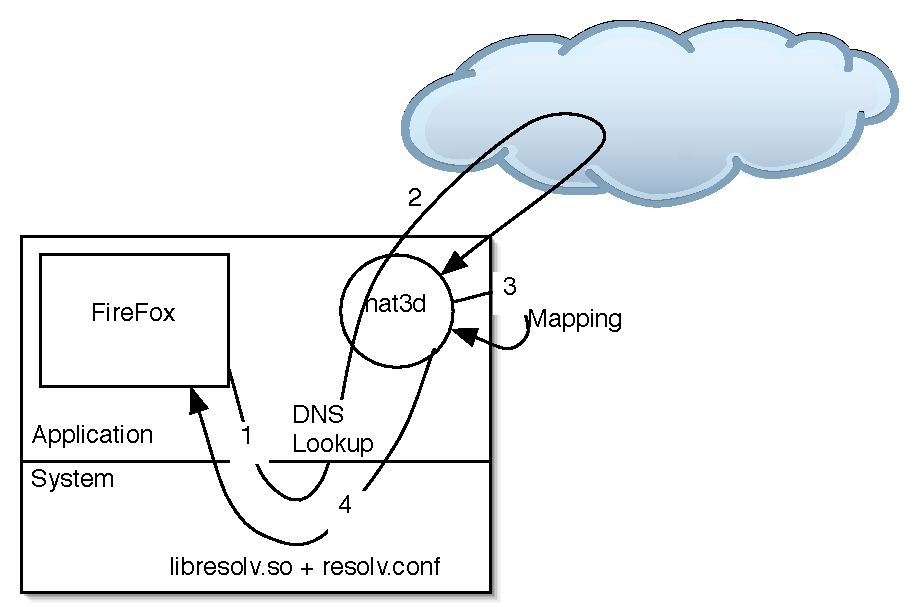
\includegraphics[width=0.9\textwidth]{figs/dns-control-flow}
\end{center}
\caption{DNS control flow}
\label{fig:dns-control-flow}
\end{figure}

The DNS Resolver component intercepts all DNS requests issued by the user and will forward them to the network's local caching resolver.  When
that resolver gets an NXDOMAIN back for an A record query, the NATTT resolver re-issues the same query, but specifies the NAT3 RR type.
This allows NAT3 to see if there is a fallback connection to a destination.

If the NAT3 request finds RRs, then the other end must be behind a NAT box.  At this point the resolver communicates with the Tunnel Manger 
in order to create a tunnel through the remote NAT box.  This is depicted in Figure~\ref{fig:dns-control-flow}

\subsection{Tunnel Manager}

\begin{figure}
\begin{center}
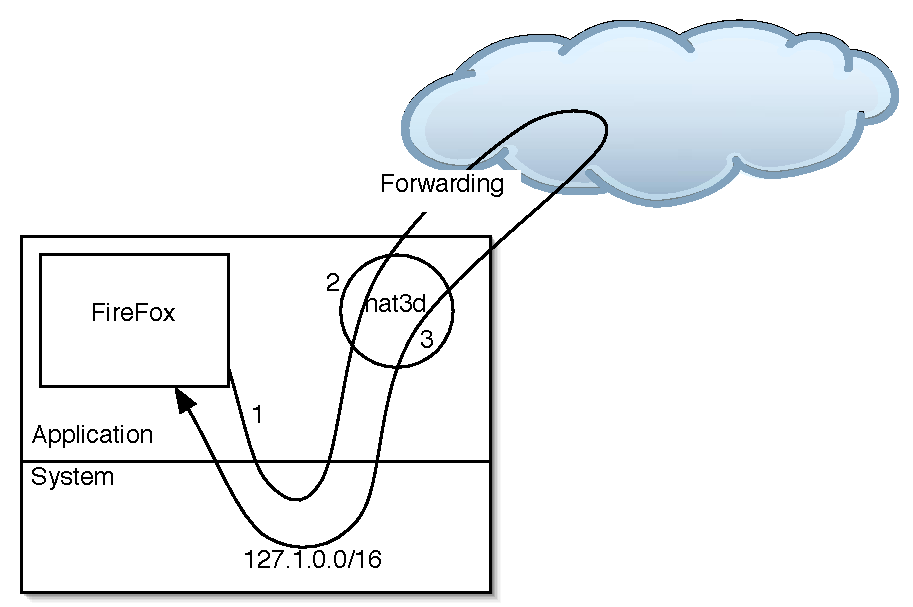
\includegraphics[width=0.9\textwidth]{figs/tun-control-flow}
\end{center}
\caption{Tunnel Manager control flow}
\label{fig:tun-control-flow}
\end{figure}

The Tunnel Manager is responsible for the network-layer communications between a local application (such as FireFox) and a remote
destination that may be behind a NAT box.  The tunnel manager creates and maintains a cache of tunnels that are in use.  

{\bf Outbound Traffic:} All traffic that is
to be sent through the tunnel is captured by the Tunnel Manger and encapsulated.  Specifically, all packets (TCP and UDP) are encapsulated
into UDP datagrams.  The IP header of the datagram contains the information about the public address of the remote NAT.  The datagram then
has a second (encapsulated) IP header that specifies the \emph{internal} address of the  destination.  The local (source) information in
each header is the local (internal) IP address of the user's host.  As the packet traverses the local NAT box (if there is one), the outer
header will have its address re-written.  When the Tunnel Manager needs
to create a new tunnel, it allocates a new IP address inside of the $127.1.0.0/16$ subnet and creates a mapping for this new IP and the 
outbound port used to actually send the packet.  This is a subnet that the Tunnel Manager accepts
all local traffic from (on the individual) machine.  By using this network, the Tunnel Manager can assign its own locally routable addresses
without worrying about potential address conflicts (because $127.0.0.0/8$ is defined to be a non-routable prefix).  These IP addresses can 
then be used by 3rd party applications as a tunnel ingress in place of the remote destination.  Thus, applications like FireFox are given an
IP address that is unique to a local tunnel, and the tunnel manager intercepts all traffic and encapsulates it.  

{\bf Inbound Traffic:} All inbound traffic is received by the tunnel manager on a specific port that it listens on.  When traffic is received
for the Tunnel Manager, its external and internal headers are used to identify if there is an existing tunnel from the remote source, and if
no tunnel mapping exists, a new one is created.  The tunnel mapping indicates a specific local IP address (in the $127.1.0.0/16$ subnet) 
to use as the source address when re-writing the inbound packet.  This way, the client (such as FireFox) will respond to a local IP address
that the Tunnel Manager will intercept and can then rewrite the packet for.

This is depicted in Figure~\ref{fig:tun-control-flow}.
